\documentclass[12pt]{article}

\usepackage[utf8]{inputenc}
\usepackage{EngReport}
\usepackage{listings}
\usepackage{cancel}
\usepackage{comment}
\usepackage{amssymb}
\usepackage{amsthm}
\usepackage{amsmath}
\usepackage{graphicx}
\usepackage{setspace}
\usepackage{geometry}
\usepackage{xcolor}  % Required for coloring in listings
\usepackage{tikz}

\graphicspath{{Images/}}
\onehalfspacing
\geometry{letterpaper, portrait, includeheadfoot=true, hmargin=1in, vmargin=1in}

% Define custom colors
\definecolor{myblue}{RGB}{0, 128, 255}
\definecolor{mygreen}{RGB}{34, 139, 34}
\definecolor{myorange}{RGB}{255, 140, 0}
\definecolor{mygray}{RGB}{128, 128, 128}
\definecolor{mypurple}{RGB}{148, 0, 211}
\definecolor{myred}{RGB}{255, 69, 0}

% Configure listings for Python with custom styles
\lstset{
    language=Python,             % Set language to Python
    basicstyle=\ttfamily\small,  % Use a smaller monospace font
    keywordstyle=\color{myblue}\bfseries,  % Keywords in blue and bold
    commentstyle=\color{mygreen}\itshape,  % Comments in green and italic
    stringstyle=\color{myorange},          % Strings in orange
    numberstyle=\color{mygray},            % Line numbers in gray
    identifierstyle=\color{mypurple},      % Functions and variables in purple
    morekeywords={print, len, range},      % Define additional Python keywords
    showstringspaces=false,                % Do not show spaces in strings
    breaklines=true,                       % Enable line breaking
    numbers=left,                          % Add line numbers to the left
    numbersep=5pt,                         % Space between line numbers and code
    frame=single,                          % Add a box around the code
    rulecolor=\color{mygray},              % Frame color
    moredelim=[is][\color{myred}]{@@}{@@}, % Custom inline LaTeX coloring
}

\begin{document}
\renewcommand{\familydefault}{\rmdefault}

\begin{titlepage}
    \null % This is a TeX command that does nothing but is necessary for vfill to work correctly
    \vfill
    \begin{center}
        {\fontsize{35}{48}\selectfont \bfseries CSC263 Tutorial \#1 Exercises}
        \vspace{20pt} \\
        {\LARGE Analyzing the Worst, Best, and Average Max Function} \\
        \vspace{20pt}
        \textbf{Alexander He Meng}
        \vspace{8pt}
        \\ Prepared for January 10, 2025
    \end{center}
    \vfill
\end{titlepage}

\pagestyle{fancy}
\fancyhf{}
\setlength{\headheight}{30pt}
\renewcommand{\headrulewidth}{0.4pt}
\renewcommand{\footrulewidth}{0.4pt}
\lhead{\large \textbf{CSC263 UTM} \\ \textbf{Tutorial 3 Exercises}}
\rhead{\large \textbf{Winter 2025} \\ \textbf{Due Jan 2025}}
\rfoot{\textbf{Page \thepage}}
\lfoot{}
\pagebreak
\normalsize

\section*{Question \#1}
\textbf{\underline{Claim:}} The \textit{minimum} element of a binary max-heap must be one of its leaf nodes (assuming distinct elements).

\begin{proof}
\leavevmode\\
Seeking a contradiction, assume the minimum element of a binary max-heap is not a leaf node. Then, it must have at least one child node. \\
Since this element is the minimum, that child node must contain a larger element, and this contradicts the property of a binary max-heap where parent nodes are larger than their children. \\
By this contradiction, the minimum element of a binary max-heap must be one of its leaf nodes. \\
\end{proof}
\pagebreak

\section*{Question \#2}
\textbf{\underline{Claim:}} The \textit{median} element of a binary max-heap is \textbf{not necessarily} one of its leaf nodes.

\begin{proof}
\leavevmode\\
Consider the binary max-heap \texttt{max\_heap = [5, 3, 4, 2, 1]}, represented as:
\\
\begin{center}
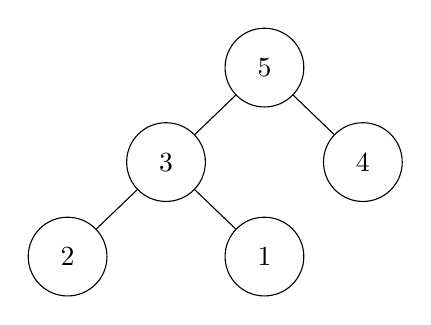
\begin{tikzpicture}[level distance=1.2cm, sibling distance=2.5cm,
  every node/.style={circle, draw, minimum size=1cm, inner sep=0}]
  
  % Root node
  \node {5}
    % Level 1
    child {node {3}
      % Level 2
      child {node {2}}
      child {node {1}}
    }
    child {node {4}
    };
\end{tikzpicture}
\end{center}
Clearly, the median element is \texttt{3}, yet it is not a leaf node. \\
\end{proof}
\pagebreak

\section*{Question \#3}
A ternary max-heap is like a binary max-heap except that non-leaf nodes have three children instead of two children. (As with binary heaps, there can of course be one non-leaf node that has fewer than three children.) We refer to the children as the left child, middle child, and right child.

The values stored in the nodes are ordered according to the same principle as for binary max-heaps: the value at each node is greater than or equal to the values in the node’s children. Answer the following questions regarding ternary max-heaps:

\subsection*{(a)}
\textbf{\underline{Claim:}} In a ternary max-heap, the indices of the left, middle, and right children are \(3i + 1\), \(3i + 2\), and \(3i + 3\), respectively.
\begin{proof}
\leavevmode\\
Given the array representation of the ternary heap, for any node at index \(i\):
\begin{itemize}
    \item The left child is located at \(3i + 1\).
    \item The middle child is located at \(3i + 2\).
    \item The right child is located at \(3i + 3\).
\end{itemize}
These formulas arise from the structure of the array representation of a complete ternary tree. For corner cases:
\begin{itemize}
    \item If \(3i + 1\), \(3i + 2\), or \(3i + 3\) exceed the array length, the node has fewer than three children.
\end{itemize}
\end{proof}

\subsection*{(b)}
\textbf{\underline{Claim:}} In a ternary max-heap, \texttt{EXTRACT-MAX} works by removing the root node and replacing it with the last element of the heap, then “bubbling down” to restore the max-heap property. \texttt{INSERT} works by appending the new element to the end of the array and “bubbling up” to restore the max-heap property.
\begin{proof}
\leavevmode\\
The differences from binary max-heaps are primarily in handling three children instead of two during the bubbling operations. For \texttt{EXTRACT-MAX}, during bubbling down, the parent node is swapped with the largest of its three children if it violates the max-heap property. For \texttt{INSERT}, during bubbling up, the inserted node is swapped with its parent if it is larger than the parent.
\end{proof}

\subsection*{(c)}
\textbf{Recursive Implementation:}
\begin{lstlisting}
IS_TERNARY_MAX_HEAP(A: list[int], i: int) -> bool:
    if 3i + 1 >= len(A):  # Node has no children
        return True

    left = 3i + 1
    middle = 3i + 2
    right = 3i + 3

    # Check max-heap property
    if (left < len(A) and A[i] < A[left]) or \
       (middle < len(A) and A[i] < A[middle]) or \
       (right < len(A) and A[i] < A[right]):
        return False

    return IS_TERNARY_MAX_HEAP(A, left) and \
           IS_TERNARY_MAX_HEAP(A, middle) and \
           IS_TERNARY_MAX_HEAP(A, right)
\end{lstlisting}
\textbf{Explanation:} The function checks the max-heap property at the current node and recursively verifies the children. The worst-case runtime is \(O(n)\).

\subsection*{(d)}
\textbf{Iterative Implementation:}
\begin{lstlisting}
IS_TERNARY_MAX_HEAP_ITER(A: list[int]) -> bool:
    for i in range(len(A)):
        left = 3i + 1
        middle = 3i + 2
        right = 3i + 3

        if (left < len(A) and A[i] < A[left]) or \
           (middle < len(A) and A[i] < A[middle]) or \
           (right < len(A) and A[i] < A[right]):
            return False

    return True
\end{lstlisting}
\textbf{Explanation:} The iterative approach checks each node in a loop. The worst-case runtime is \(O(n)\).

\end{document}
